%
% FIX THIS -- remove/change, just some examples of things
%


\chapter{Partially Observable Environments}

\section{Introduction}
%this is how an image should look
%\includegraphics{universe}
Until now, both the GTGR and GTGRD models have given the observer full knowledge of the adversary's state for the entirety of the game. In real-world environments, observers may not have perfect information regarding the states and actions of an adversary. 


To accommodate for scenarios with incomplete information for the adversary, we introduce a partially observable variant of the GTGR scenario. In partially observable scenarios, the rules of the game remain largely unchanged, except for addition of “shadow states." The observer can not discern the current state of the adversary, while the adversary occupies a shadow state. When the adversary enters an observable portion of the graph, the observer will become aware of the adversary's position once more.

\begin{figure}[h!]
\begin{center}

  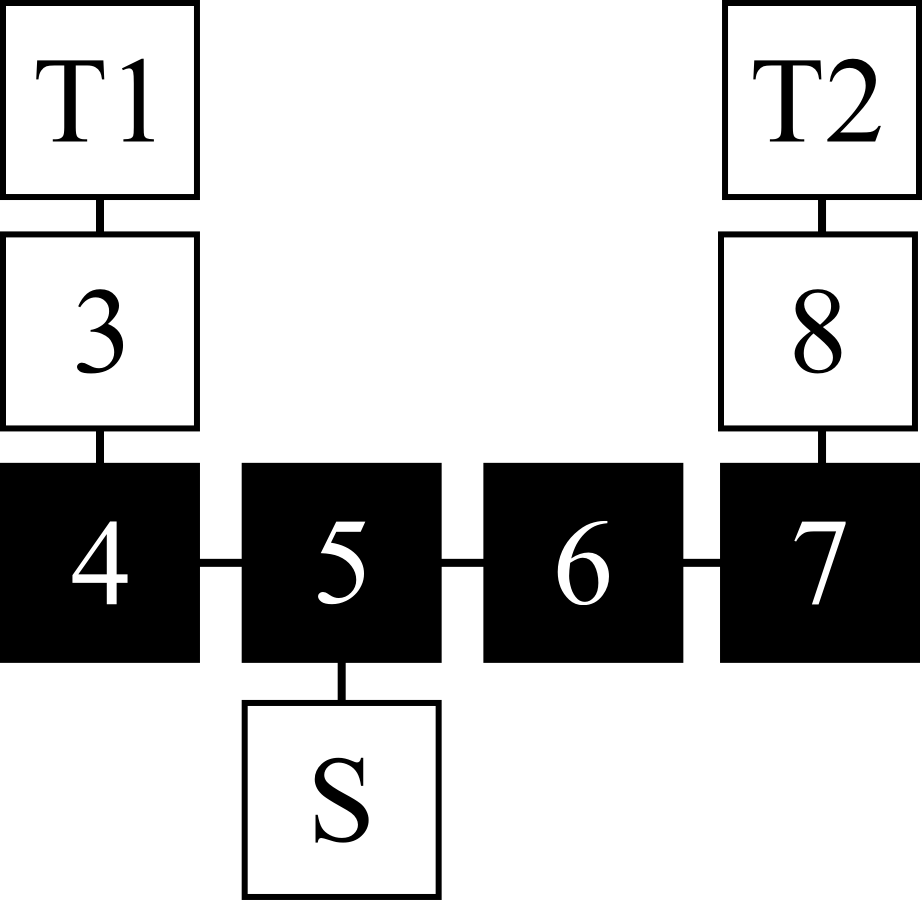
\includegraphics[scale=.25]{shadow1}
  \end{center}

  \caption{A partially observable graph.}
  \label{fig:shadow1}
\end{figure}

Figure~\ref{fig:shadow1} illustrates a partially observable environment. Visible states, in which the observer can see the adversary  white. Shadow states, in which the adversary is hidden from the observer, are black. The agent starts the game in state $S$. When the adversary moves to states $4$ ,$5$, $6$, or $7$, the observer is unable to determine their position until the adversary re-enters a visible portion of the graph.  
We will examine two solutions to the partially observable model, both of which involving linear programming. 

\section{The Whale Method}

The first method solving these partially observable environments will utilize disjoint sets of shadow states. We call these collections "shadow sets." We say that two shadow states belong to the same shadow set, if the adversary can travel between the two without entering an observable state.

In the example illustrated in Figure~\ref{fig:shadow1}, when the adversary moves to nodes 4, 5, or 7 (the three entrance points to the hidden portion of the graph) the observer will only know that the adversary has entered the state Z1. From the observer’s point of view, the adversary will remain in Z1 until the adversary moves to nodes, 3, 8, or S, (the three exit points from the hidden portion of the graph). When the adversary enters Z1, the observer knows what states the adversary could possibly occupy without directly observing them. With the fat solution, the observer takes the same action for every turn the adversary spends in a hidden portion of the graph. We can easily modify the linear program to accommodate the fat solution.

\begin{equation}
max_{V, \{f_i(s)\}_{i,s}} \sum_{\theta} P(\theta)V(\theta, s_o) \tag{2}
\end{equation}

\begin{equation}
V(\theta, s) \leq \sum_{i \in B} r(s, i, j, \theta)f_{i}(s) + V(\theta, j) \forall\theta\in B,\forall s \mid s\neq \theta, \forall j\in\nu(s) \tag{3}
\end{equation}

\begin{equation}
V(\theta, s) = 0 \quad \mbox{when} \ s=\theta \tag{4}
\end{equation}

\begin{equation}
\sum_{i} f_{i}(s) = 1\quad \forall s \tag{3}
\end{equation}

\begin{equation}
f_{i}(s) \geq 0\quad \forall s,i\
\end{equation}
\nocite{Dijkstra80}
\nocite{plop03-paper}
